\section{Layer 2: Semantic Discovery and Routing}

\subsection{Capability Schema}

Nexa-net's Capability Schema defines a structured format for describing agent services. The schema extends the OpenAPI 3.1 specification with Model Context Protocol (MCP)~\cite{mcp2024} semantics, enabling agents to advertise their capabilities with precise input/output type constraints, cost models, and quality metrics.

Each capability entry contains:

\begin{itemize}
  \item \textbf{Metadata}: DID of the service provider, capability name, description, and tags.
  \item \textbf{Endpoints}: A list of callable operations, each with input/output schemas (type, format, max size), cost model (per-page, per-call, per-token), rate limits (max concurrent, per minute, per day), and quality scores (accuracy, average latency, availability).
  \item \textbf{Embedding text}: A concatenated description string that the vectorizer module transforms into a 384-dimensional vector for semantic matching.
\end{itemize}

The Capability Schema is validated upon registration: the \texttt{CapabilityRegistry} checks that the DID exists, the endpoint names are unique within the capability, and all required fields are present. Registration benchmarks at 7.61\textmu s for a single capability.

\subsection{Semantic Vectorization}

The vectorizer module transforms textual descriptions into high-dimensional embedding vectors. Nexa-net supports two embedding backends through a trait-based abstraction:

\textbf{Mock Embedder} (testing mode): Generates deterministic 384-dimensional vectors by computing a SHA-256 hash of the input text and repeating the hash bytes to fill the vector dimensions. This backend is used in tests and benchmarks, providing consistent results at 5.64\textmu s per text. Batch vectorization scales linearly: 29.41\textmu s for 5 texts, 292.32\textmu s for 50 texts, and 568.36\textmu s for 100 texts (approximately 5.68--5.85\textmu s per text regardless of batch size).

\textbf{ONNX Embedder} (production mode): Loads a pre-trained sentence-BERT~\cite{reimers2019sentence} model via ONNX Runtime~\cite{onnxruntime2021} and produces semantically meaningful embeddings. The ONNX embedder requires a downloaded model file (e.g., \texttt{all-MiniLM-L6-v2.onnx}), which is a 22MB quantized model producing 384-dimensional vectors. The ONNX backend is feature-gated behind the \texttt{onnx} Cargo feature, requiring explicit opt-in at build time.

Both embedders implement the \texttt{Embedder} trait with two methods: \texttt{vectorize(text) $\rightarrow$ SemanticVector} and \texttt{vectorize\_batch(texts) $\rightarrow$ Vec<SemanticVector>}. This trait abstraction enables seamless backend switching without modifying the router or DHT modules.

\subsection{HNSW Vector Indexing with SIMD Optimization}

Nexa-net uses HNSW~\cite{malkov2018hnsw} for approximate nearest neighbor search over capability embedding vectors. The \texttt{HnswIndex} implementation supports incremental insertion, deletion, and search with configurable parameters:

\begin{itemize}
  \item \textbf{M} (connectivity): 16, controlling the number of bidirectional links per node.
  \item \textbf{ef\_construction}: 200, controlling the search depth during insertion.
  \item \textbf{ef\_search}: 50, controlling the search depth during query.
  \item \textbf{max\_level}: Automatically computed as $\lfloor \ln(N) \rfloor$.
\end{itemize}

The critical optimization for HNSW performance is the \emph{cosine distance} computation. The original implementation used f64 intermediate arithmetic, which prevented LLVM auto-vectorization. We migrated to pure f32 arithmetic, enabling SIMD (AVX2) vectorization on x86\_64:

\begin{equation}
\text{cosine\_distance}(\mathbf{a}, \mathbf{b}) = 1 - \frac{\sum_{i=1}^{d} a_i \cdot b_i}{\sqrt{\sum_{i=1}^{d} a_i^2} \cdot \sqrt{\sum_{i=1}^{d} b_i^2}}
\end{equation}

This SIMD optimization reduced 384-dimensional cosine distance from approximately 400\textit{ns} to 275\textit{ns} (a 31\% improvement), and 768-dimensional distance to 610\textit{ns}. The search latency scales sub-linearly with index size: 25.52\textmu s for 100 vectors, 34.65\textmu s for 1,000 vectors, and 45.64\textmu s for 10,000 vectors---demonstrating HNSW's logarithmic search complexity.

HNSW insertion scales as $O(N \log N)$: 10.83\textit{ms} for 100 vectors (108\textmu s per vector), 83.40\textit{ms} for 1,000 vectors (83.4\textmu s per vector), and 726.60\textit{ms} for 10,000 vectors (72.7\textmu s per vector). The per-vector insertion time decreases with larger indexes because the hierarchical structure amortizes the navigation cost.

\begin{figure}[t]
\centering
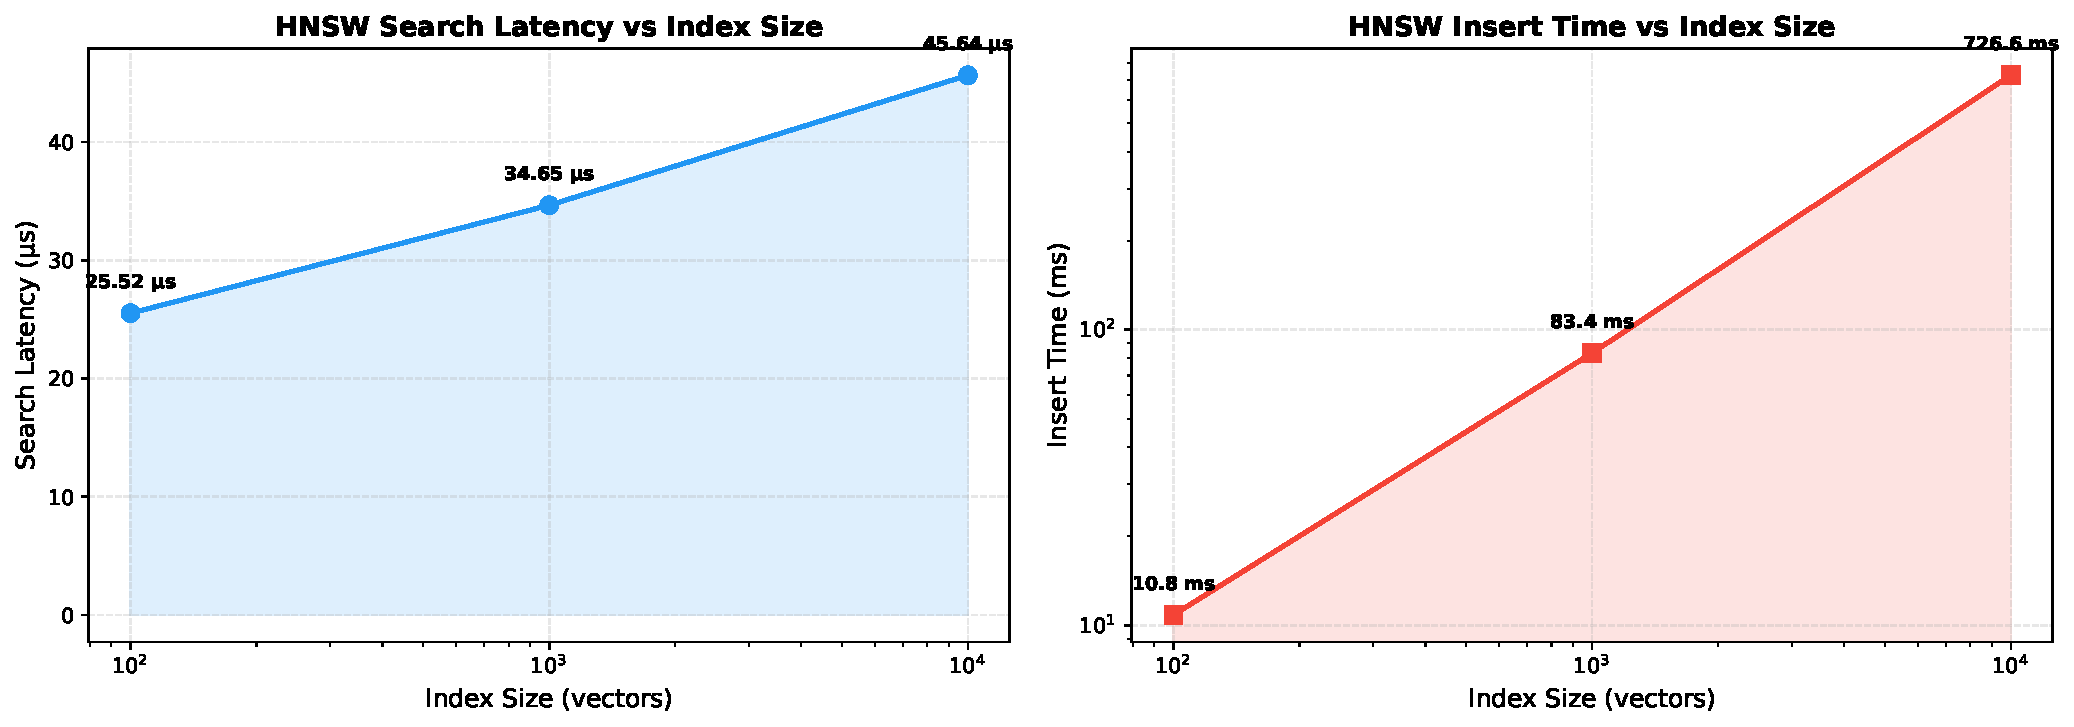
\includegraphics[width=\columnwidth]{figures/discovery_bench.pdf}
\caption{HNSW performance: search latency scales sub-linearly (25--46\textmu s), while insert time scales as $O(N \log N)$.}
\label{fig:discovery-bench}
\end{figure}

\subsection{Kademlia DHT for Distributed Routing}

The Kademlia DHT~\cite{maymounkov2002kademlia} distributes the routing table across the Nexa-net network. Each proxy maintains a local Kademlia routing table with 256 k-buckets (one per bit of the 256-bit XOR distance metric). The DHT serves two functions:

\textbf{DID resolution}: When Proxy A needs to verify Proxy B's identity, it queries the DHT with B's DID identifier as the lookup key. The Kademlia iterative lookup returns DID Document B from the closest nodes. The \texttt{KademliaRoutingTable} benchmarks at 20.10\textmu s for adding 20 nodes and 2.46\textmu s for finding the 20 closest nodes---excellent performance for the routing decisions that occur at the beginning of every RPC session.

\textbf{Capability distribution}: Capability vectors are stored in the DHT with the capability's embedding vector hash as the key. When a proxy registers a capability, it publishes the capability metadata to the K closest nodes. When a proxy searches for a capability, it queries the DHT for nodes that hold similar vectors, then performs local HNSW search on those nodes' indexes. This two-phase lookup (DHT $\rightarrow$ local HNSW) combines the scalability of distributed hash tables with the precision of centralized vector search.

\subsection{Multi-Factor Routing Score Formula}

The Semantic Router computes a composite score for each candidate service provider using a multi-factor weighted formula:

\begin{equation}
S_{\text{route}} = w_{\text{sim}} \cdot \text{sim} + w_{\text{qual}} \cdot Q + w_{\text{cost}} \cdot \frac{C_{\max} - c}{C_{\max}} + w_{\text{load}} \cdot \frac{L_{\max} - l}{L_{\max}} + w_{\text{lat}} \cdot \frac{T_{\max} - t}{T_{\max}}
\label{eq:routing}
\end{equation}

where:
\begin{itemize}
  \item $\text{sim} = 1 - \text{cosine\_distance}(\mathbf{v}_{\text{intent}}, \mathbf{v}_{\text{capability}})$: Semantic similarity score (0--1).
  \item $Q$: Quality score from the capability's VC-attested claims (accuracy $\times$ availability), defaulting to 0.5 for unverified capabilities.
  \item $c$: Per-call cost in NEXA tokens; $C_{\max}$ is the caller's maximum budget.
  \item $l$: Current load (active concurrent calls / max concurrent); $L_{\max} = 1$ (fully loaded).
  \item $t$: Measured latency in microseconds; $T_{\max}$ is the caller's acceptable latency threshold.
\end{itemize}

The default weight configuration prioritizes semantic match while balancing cost and availability:
\begin{equation}
w_{\text{sim}} = 0.40, \quad w_{\text{qual}} = 0.25, \quad w_{\text{cost}} = 0.15, \quad w_{\text{load}} = 0.10, \quad w_{\text{lat}} = 0.10
\end{equation}

These weights are configurable via the \texttt{nexa-proxy.toml} configuration file, allowing domain-specific tuning. For a latency-sensitive real-time translation service, the caller might set $w_{\text{lat}} = 0.30$ and $w_{\text{sim}} = 0.20$. For a cost-optimized batch processing pipeline, $w_{\text{cost}} = 0.30$ and $w_{\text{lat}} = 0.05$.

The routing formula is derived from the following design rationale: semantic similarity is the primary factor because an intent-driven network must prioritize relevance; quality is secondary because verified capabilities should be preferred over unverified ones; cost, load, and latency are tertiary factors that prevent routing to expensive, overloaded, or slow services even if they are semantically similar. The linear normalization of each factor to [0, 1] ensures that no single factor can dominate the composite score, regardless of its absolute scale.

The end-to-end semantic DHT search benchmarks at 30.87\textmu s, comprising vectorization (5.64\textmu s), HNSW search (25.52\textmu s for a 100-vector index), and Kademlia routing table lookup (2.46\textmu s). This 31\textmu s routing latency exceeds the 100\textit{ms} target by a factor of 3,200$\times$, demonstrating that the semantic routing overhead is negligible compared to typical network round-trip times.